\documentclass[border=4pt]{standalone}

\usepackage{pgfplots}
\usepackage{pgfplotstable}
\pgfplotsset{compat=1.18, width=8.5cm, height=5.6cm, tick label style={font=\small}, label style={font=\small}, legend cell align=left, legend style={font=\small, draw=none, fill=none}}

\definecolor{plnavy}{HTML}{1F4E89}
\definecolor{plrose}{HTML}{B85A52}
\definecolor{plsage}{HTML}{93CC9E}
\definecolor{plsand}{HTML}{E0BE78}
\definecolor{plplum}{HTML}{8E7BB5}
\definecolor{plgray}{HTML}{6E6E6E}

% ==== parameters: curve centers, widths and the annotated gap ====
\def\muA{-0.40}  \def\widthA{0.13}
\def\muB{-0.40}  \def\widthB{0.24}  \def\heightB{0.30}  \def\floorB{0.22}
\def\muC{0.43}   \def\widthC{0.12}
\newcommand{\curveA}{$P(y \mid x)$}
\newcommand{\curveB}{$P(y \mid \tilde{x})$}
\newcommand{\curveC}{$P(y \mid x, z)$}
\newcommand{\gaplabel}{Gain}

\begin{document}
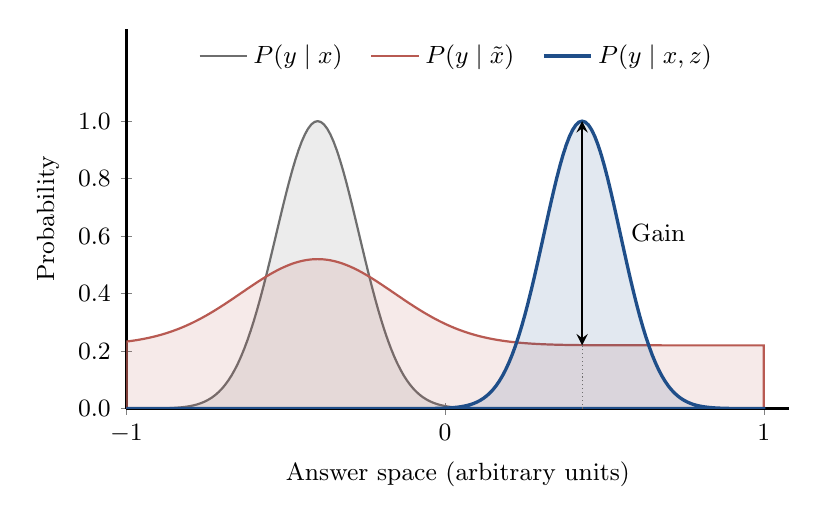
\begin{tikzpicture}
\begin{axis}[width=10cm, height=6.4cm, axis lines=left, axis line style={line width=1.1pt, -}, xmin=-1, xmax=1.08, ymin=0, ymax=1.32, xtick={-1,0,1}, ytick={0,0.2,...,1}, xlabel={Answer space (arbitrary units)}, ylabel={Probability}, domain=-1:1, samples=201, no markers, declare function={bump(\x,\m,\s)=exp(-0.5*((\x-\m)/\s)^2);}, legend style={at={(0.5,0.99)}, anchor=north, legend columns=3, /tikz/every even column/.append style={column sep=8pt}}, yticklabel style={/pgf/number format/fixed, /pgf/number format/precision=1, /pgf/number format/fixed zerofill}]
  \addplot[draw=plgray, thick, fill=plgray, fill opacity=0.13, draw opacity=1] {bump(x,\muA,\widthA)} \closedcycle;
  \addlegendentry{\curveA}
  \addplot[draw=plrose, thick, fill=plrose, fill opacity=0.13, draw opacity=1] {\floorB*(1-bump(x,\muB,\widthB))+(\heightB+\floorB)*bump(x,\muB,\widthB)} \closedcycle;
  \addlegendentry{\curveB}
  \addplot[draw=plnavy, line width=1.2pt, fill=plnavy, fill opacity=0.13, draw opacity=1] {bump(x,\muC,\widthC)} \closedcycle;
  \addlegendentry{\curveC}
  \draw[<->, >=stealth, thick] (axis cs:\muC,\floorB) -- (axis cs:\muC,1) node[midway, right=14pt, font=\small] {\gaplabel};
  \draw[densely dotted, plgray] (axis cs:\muC,0) -- (axis cs:\muC,\floorB);
\end{axis}
\end{tikzpicture}
\end{document}
